\documentclass{article}
\usepackage{tikz}
\usetikzlibrary{shapes, arrows.meta, calc, positioning}

\begin{document}

\begin{figure}[htbp]
\centering
\resizebox{\textwidth}{!}{
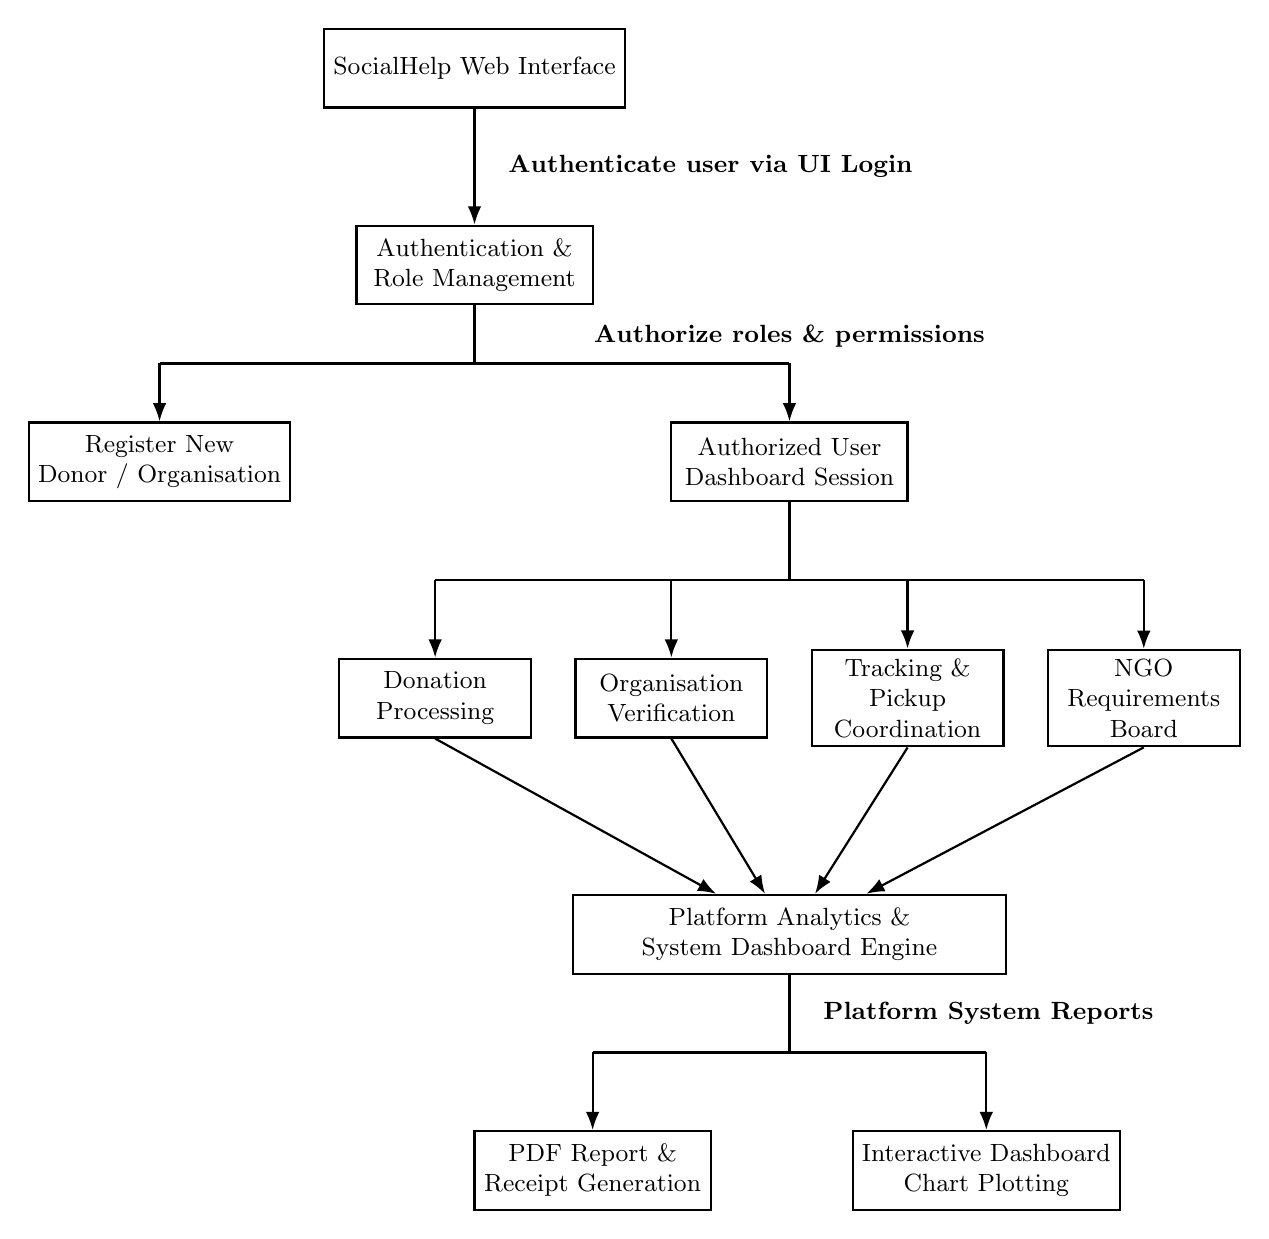
\begin{tikzpicture}[
    >=Latex,
    block/.style={draw, rectangle, minimum width=3cm, minimum height=1cm, align=center, font=\small, fill=white, thick},
    labelStyle/.style={font=\small\bfseries, align=left, text=black}
]

% ----------------------------------------------------
% Level 0 & 1 (Main Entrance)
% ----------------------------------------------------
\node[block] (UI) at (1, 0) {SocialHelp Web Interface};

\node[block] (Auth) at (1, -2.5) {Authentication \&\\Role Management};

\draw[->, thick] (UI.south) -- (Auth.north) 
    node[midway, right=0.3cm, labelStyle] {Authenticate user via UI Login};

% ----------------------------------------------------
% Level 2 (Registration vs Authorized Session Fork)
% ----------------------------------------------------
\node[block] (Register) at (-3, -5) {Register New\\Donor / Organisation};
\node[block] (SuccessAuth) at (5, -5) {Authorized User\\Dashboard Session};

% T-Fork 1 (Perfectly symmetric orthogonal fork from x=1 to -3 and 5)
\draw[-, thick] (Auth.south) -- (1, -3.75);
\draw[-, thick] (-3, -3.75) -- (5, -3.75);
\draw[->, thick] (-3, -3.75) -- (Register.north);
\draw[->, thick] (5, -3.75) -- (SuccessAuth.north);

\node[labelStyle] at (5, -3.4) {Authorize roles \& permissions};

% ----------------------------------------------------
% Level 3 (The 4 Core Social Help Functional Modules)
% ----------------------------------------------------
\node[block, text width=2.2cm, minimum width=2.4cm] (M1) at (0.5, -8) {Donation\\Processing};
\node[block, text width=2.2cm, minimum width=2.4cm] (M2) at (3.5, -8) {Organisation\\Verification};
\node[block, text width=2.2cm, minimum width=2.4cm] (M3) at (6.5, -8) {Tracking \&\\Pickup\\Coordination};
\node[block, text width=2.2cm, minimum width=2.4cm] (M4) at (9.5, -8) {NGO\\Requirements\\Board};

% 4-Way Fork (Symmetrically branching downwards from x=5)
\draw[-, thick] (SuccessAuth.south) -- (5, -6.5);
\draw[-, thick] (0.5, -6.5) -- (9.5, -6.5);
\draw[->, thick] (0.5, -6.5) -- (M1.north);
\draw[->, thick] (3.5, -6.5) -- (M2.north);
\draw[->, thick] (6.5, -6.5) -- (M3.north);
\draw[->, thick] (9.5, -6.5) -- (M4.north);

% ----------------------------------------------------
% Level 4 Convergence (Analytics)
% ----------------------------------------------------
\node[block, minimum width=5.5cm] (Report) at (5, -11) {Platform Analytics \&\\System Dashboard Engine};

% Slanted converging lines 
\draw[->, thick] (M1.south) -- (Report);
\draw[->, thick] (M2.south) -- (Report);
\draw[->, thick] (M3.south) -- (Report);
\draw[->, thick] (M4.south) -- (Report);

% ----------------------------------------------------
% Level 5 (Exports)
% ----------------------------------------------------
\node[block] (PDF) at (2.5, -14) {PDF Report \&\\Receipt Generation};
\node[block] (Chart) at (7.5, -14) {Interactive Dashboard\\Chart Plotting};

% T-Fork 2
\draw[-, thick] (Report.south) -- (5, -12.5) 
    node[midway, right=0.3cm, labelStyle] {Platform System Reports};
\draw[-, thick] (2.5, -12.5) -- (7.5, -12.5);
\draw[->, thick] (2.5, -12.5) -- (PDF.north);
\draw[->, thick] (7.5, -12.5) -- (Chart.north);

\end{tikzpicture}
}
\caption{Functional Decomposition Diagram (FDD) for Social Help System Architecture}
\end{figure}

\end{document}
